% Anteprima del sorgente

%% LyX 2.0.7.1 created this file.  For more info, see http://www.lyx.org/.
%% Do not edit unless you really know what you are doing.
\documentclass[twoside]{article}
\usepackage{mathpazo}
\renewcommand{\ttdefault}{mathpazo}
\usepackage[T1]{fontenc}
\usepackage[latin9]{inputenc}
\usepackage[margin={3.5cm,3.5cm}]{geometry}
\geometry{verbose,columnsep=20pt}
\usepackage{fancyhdr}
\pagestyle{fancy}
\usepackage{color}
\usepackage[unicode=true,pdfusetitle,
 bookmarks=true,bookmarksnumbered=false,bookmarksopen=false,
 breaklinks=false,pdfborder={0 0 1},backref=section,colorlinks=false]
 {hyperref}
\usepackage{breakurl}
\usepackage[pdftex]{graphicx}	
\newenvironment{Figure}
  {\par\medskip\noindent\minipage{\linewidth}}
  {\endminipage\par\medskip}

\makeatletter
\@ifundefined{date}{}{\date{}}
%%%%%%%%%%%%%%%%%%%%%%%%%%%%%% User specified LaTeX commands.
%%%%%%%%%%%%%%%%%%%%%%%%%%%%%%%%%%%%%%%%%
% Journal Article
% LaTeX Template
% Version 1.3 (9/9/13)
%
% This template has been downloaded from:
% http://www.LaTeXTemplates.com
%
% Original author:
% Frits Wenneker (http://www.howtotex.com)
%
% License:
% CC BY-NC-SA 3.0 (http://creativecommons.org/licenses/by-nc-sa/3.0/)
%
%%%%%%%%%%%%%%%%%%%%%%%%%%%%%%%%%%%%%%%%%

%----------------------------------------------------------------------------------------
%	PACKAGES AND OTHER DOCUMENT CONFIGURATIONS
%----------------------------------------------------------------------------------------



\usepackage{lipsum}% 

% Use the Palatino font
% Use 8-bit encoding that has 256 glyphs
\linespread{1.10} % Line spacing - Palatino needs more space between lines
\usepackage{microtype}% Slightly tweak font spacing for aesthetics

% Document margins
\usepackage{multicol}% Used for the two-column layout of the document
\usepackage[hang, small,labelfont=bf,up,textfont=it,up]{caption}% Custom captions under/above floats in tables or figures
% Horizontal rules in tables
% Required for tables and figures in the multi-column environment - they need to be placed in specific locations with the [H] (e.g. \begin{table}[H])
% For hyperlinks in the PDF

\usepackage{lettrine}% The lettrine is the first enlarged letter at the beginning of the text
\usepackage{paralist}% Used for the compactitem environment which makes bullet points with less space between them

\usepackage{abstract}% Allows abstract customization
\renewcommand{\abstractnamefont}{\normalfont\bfseries} % Set the "Abstract" text to bold
\renewcommand{\abstracttextfont}{\normalfont\small\itshape} % Set the abstract itself to small italic text

\usepackage{titlesec}% Allows customization of titles
\renewcommand{\thesection}{\Roman{section}} % Roman numerals for the sections
\renewcommand{\thesubsection}{\Roman{subsection}} % Roman numerals for subsections
\titleformat{\section}[block]{\large\scshape\centering}{\thesection.}{1em}{} % Change the look of the section titles
\titleformat{\subsection}[block]{\large}{\thesubsection.}{1em}{} % Change the look of the section titles

\usepackage{fancyhdr}% Headers and footers
 % All pages have headers and footers
\fancyhead{} % Blank out the default header
\fancyfoot{} % Blank out the default footer
\fancyhead[C]{CS 587 $\bullet$ December 2014} % Custom header text
\fancyfoot[RO,LE]{\thepage} % Custom footer text

%----------------------------------------------------------------------------------------
%	TITLE SECTION
%----------------------------------------------------------------------------------------

\title{\vspace{5mm}\fontsize{24pt}{10pt}\selectfont\textbf{Challenge Authentication Protocol}} % Article title

\author{
\large
\textsc{Bruzzo Paolo, Casula Dario}\\[2mm] % Your name
\normalsize University of Ilinois at Chicago \\ % Your institution
\normalsize \href{}{\{pbruzz2,dcasul3\}@uic.edu} % Your email address
\vspace{-5mm}
}


%----------------------------------------------------------------------------------------

\makeatother

\begin{document}
\maketitle 



\thispagestyle{fancy} 
\begin{abstract}
\noindent This document describes how to implement a secure and continuous
host authentication in a client-server architecture (also extendible
to a host to host authentication), through the periodic exchange of
unique and non-predictable challenges (or tokens). The Point-to-Point
Challenges Handshake Protocol (CHAP) provides protection against Replay
Attacks. The implementations of the client and the server have been
made using Python programming language.
\end{abstract}
\begin{multicols}{2} 


\section{Introduction}

Authentication is a procedure that confirms the truth of an entity which intends
to perform a given operation. Usually authentication is performed
through the exchange of a common secret. That is the core principle
of a standard password authentication protocol. This type of protocol
is vulnerable to the replay attack in which a valid data transmission
is maliciously repeated. For instance, by eavesdropping the password
(or the hash of it, which is more likely to be transmitted) an attacker can impersonate a real user and authenticate
to the server which, from that moment on, will trust the attacker
as the impersonated valid user. The Challenge-Handshake Authentication
Protocol (CHAP) provides protection against those attacks: it is used
to periodically verify the identity of a user through a 3-way handshake,
exchanging unique non-predictable session tokens. Even though the
authentication is only one-way, by implementing CHAP in both directions
it is possible a mutual authentication of the client on the server
and the server on the client.


\section{The Protocol}

The protocol is a Point-to-Point Challenge-Handshake
authentication protocol (CHAP). It is used to periodically verify
the identity of a user with a 3-way handshake. Each handshake uses
a unique challenge (session token) to authenticate the host. The answer
of the host is an hashed combination of the challenge received and
a secret, both the authenticator and host know the plaintext of the
secret. The protocol provides authentication after the link has been
already established. The authenticator starts to send a random-generated
challenge message to the host which appends the secret to the token
received and compute the hash function of the whole string. The host
sends this new message to the authenticator that checks this response
against its own computation of the expected hash value. If the two
values match, the authentication succeeds, otherwise the connection
is closed. The whole procedure, of sending a challenge, replying with
the hash and checking the response, is performed periodically in order
to keep authenticated the identity of the host, throughout the entire
session of the connection. At every cycle of execution of the algorithm,
a new different challenge is generated, in this way, all the previous
responses of the host are no more valid, since the final hash calculated
will be different. In the figure below you can see the steps of the
protocol.

\begin{Figure}
	\centering
	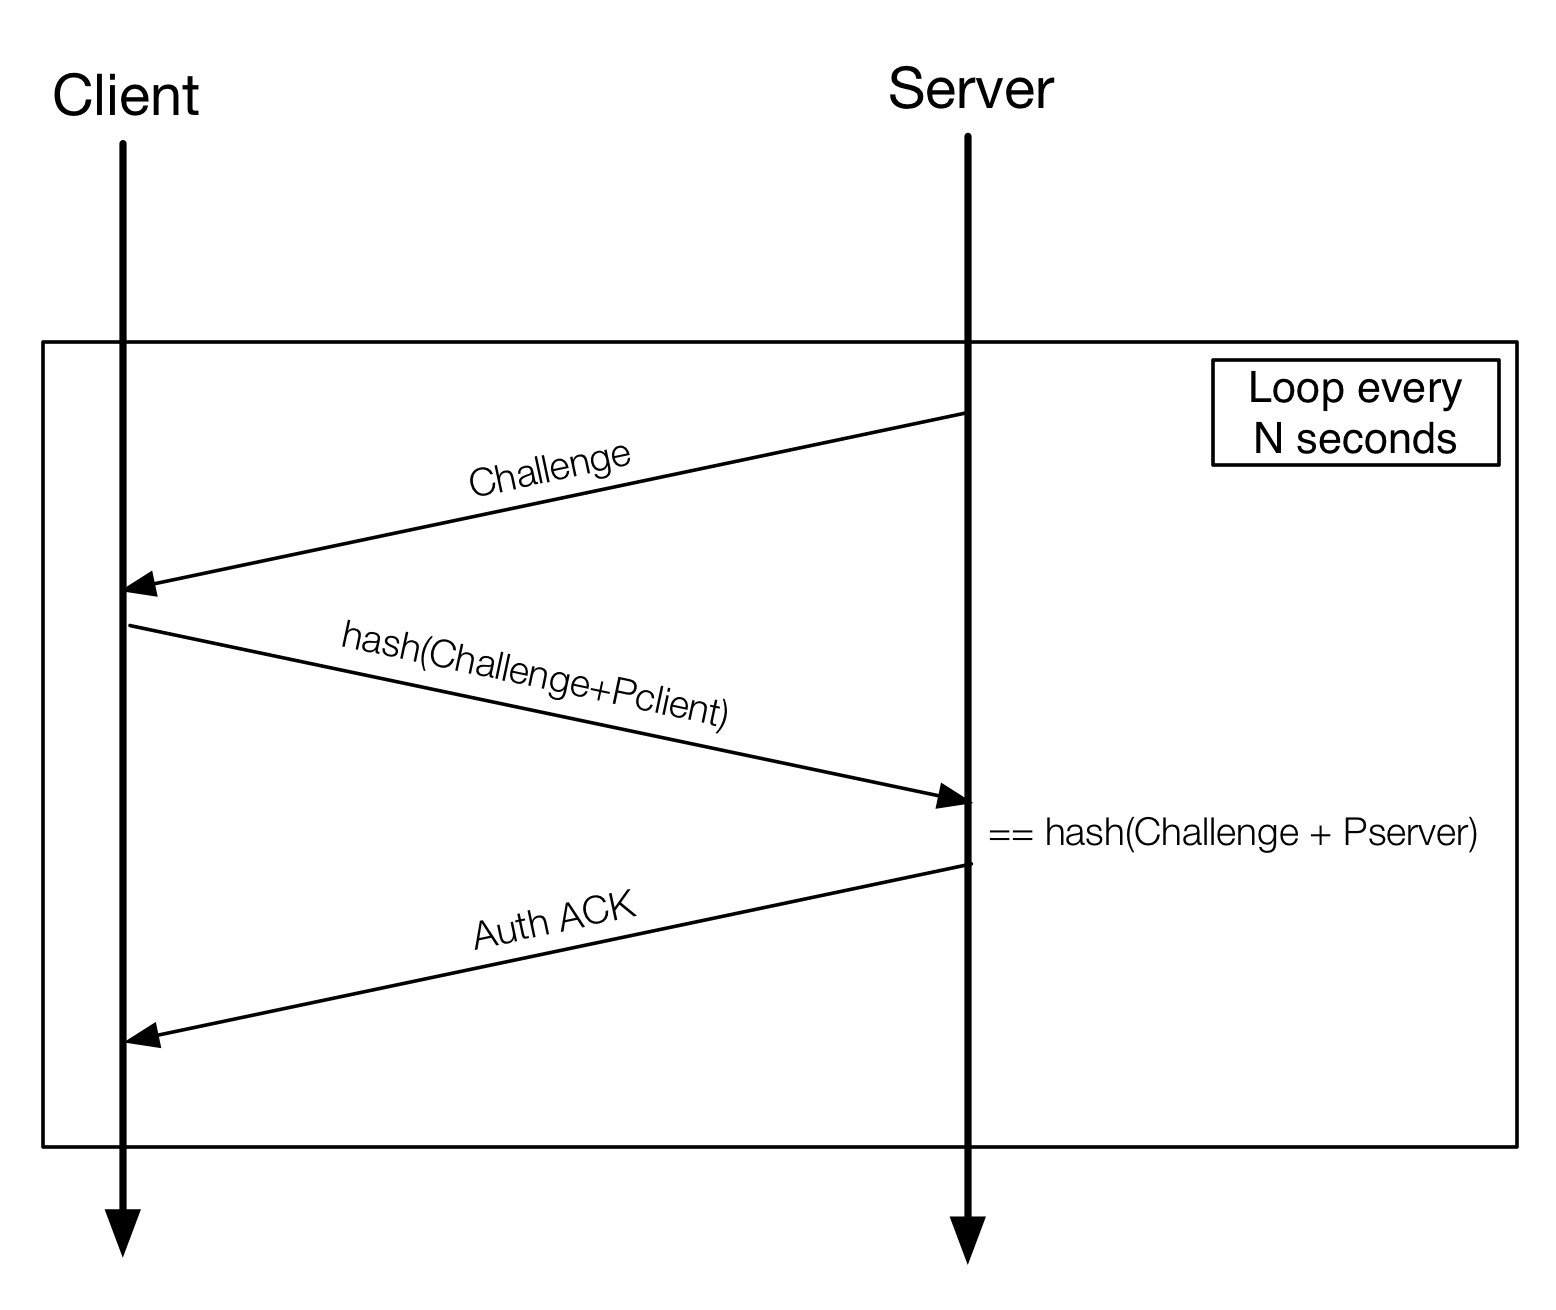
\includegraphics[width=\linewidth]{Images/Loop.png}
	\captionof{figure}{The phases of CHAP}
\end{Figure}


Here is a fast and clear summary of the steps:

\begin{compactitem} 

\item the authenticator sends a \textquotedbl{}challenge\textquotedbl{}
message to the peer;

\item the peer responds with a value calculated using a one-way hash
function on the challenge and the secret combined;

\item the authenticator checks the response against its own calculation
of the expected hash value; 

\item if the values matches, the authenticator acknowledges the authentication,
otherwise it terminates the connection;

\item at random intervals the authenticator sends a new challenge
to the host.

\end{compactitem} 


\section{The Implementation}

A client-serverconfiguration has been implemented using Python programming language.
The server is the authenticator in the CHAP protocol, while the client
is the host that has to authenticate to the server. Both the server
and the client has been implemented. The server sets up the connection
and listen to a port that will be used by the client for the authentication.
Since the protocol implemented provides protections once the link
has been already established, the server requires the client to insert
a secret that will be sent after an encoding with SHA2. If the hash
of the secret matches against the has computed by the server, the
connection is established. The CHAP protocol implement a continuous
authentication; cyclically, the server send a random-generated challenge
to the client, the client append the secret and compute the hash of
the whole message. This message is sent back to the server that checks
it and keep the connection open if the two messages match. The client
and the server start a parallel thread to handle the CHAP steps: the
server second thread sends the challenges while the client second
thread appends the secret at each handshake, encodes the message and
sends it back to the server. In the meantime, the main threads of
the client and the servers exchange messages inserted by the user.
The interval of time between two handshake is not fixed, but chosen
randomly in a range from 10 to 20 seconds. The client has in every
moment the possibility to close the connection sending a predefined
keyword that is recognized by the server.

\begin{Figure}
	\centering
	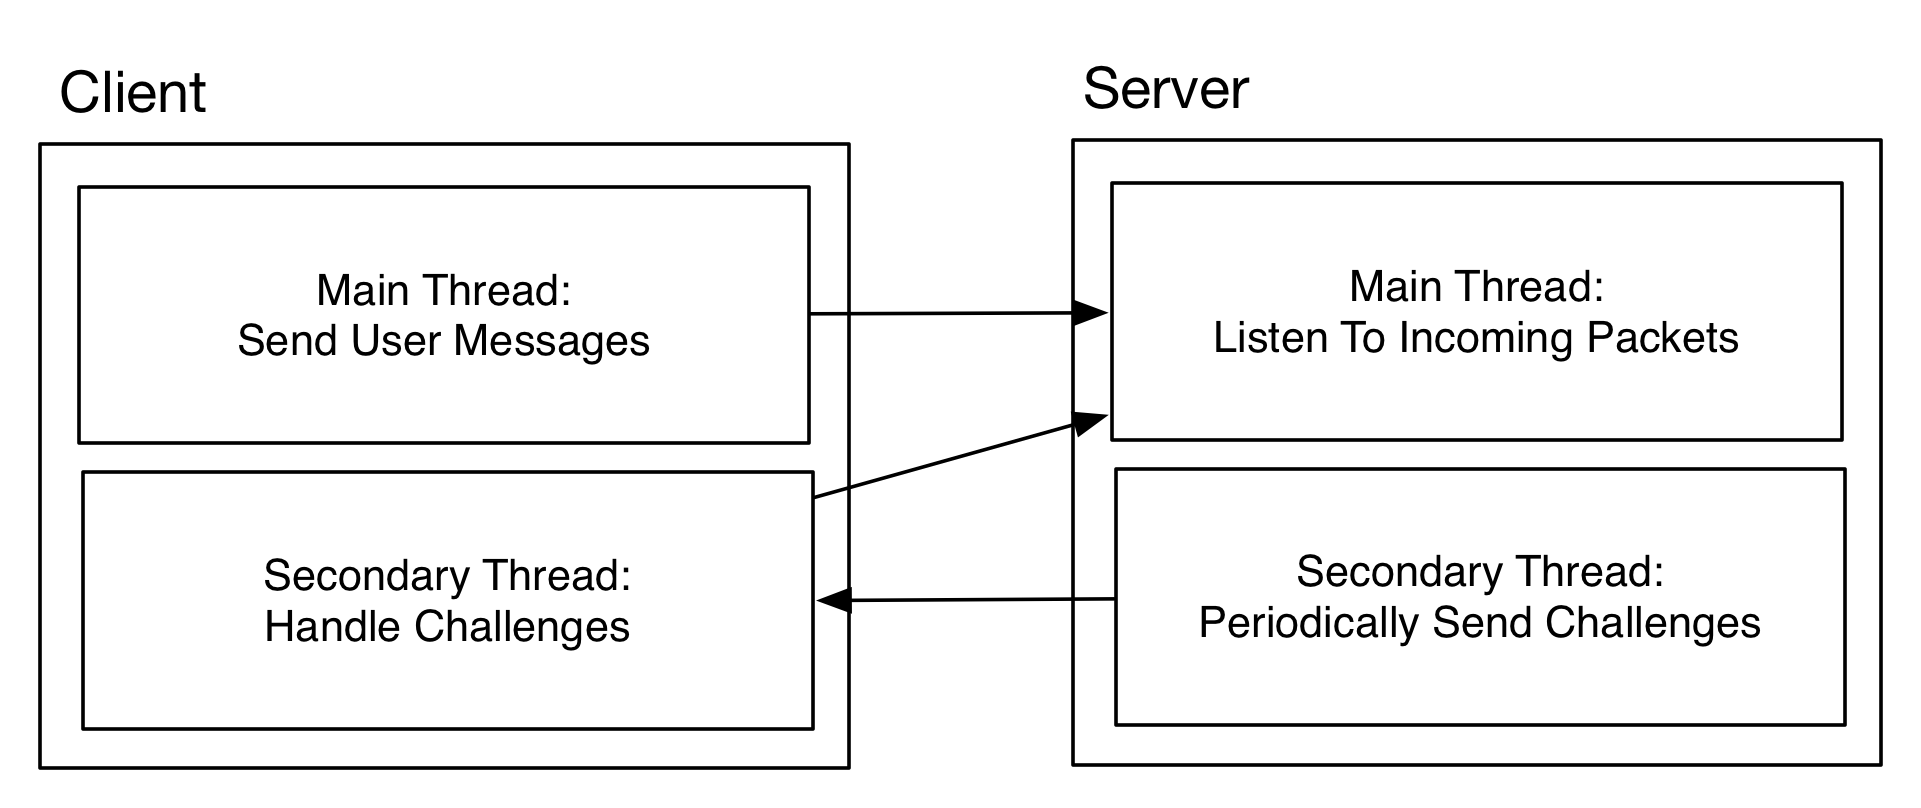
\includegraphics[width=\linewidth]{Images/Implementation.png}
	\captionof{figure}{The logic of the protocol}
\end{Figure}


\section{The protection}

The Challenge-Handshake Authentication Protocol (CHAP) provides protection
against Replay Attacks that imply eavesdropping. In the traditional
password authentication method, the connection is based on a one-time-inserted
secret that is no more checked throughout all the connection. If an
attacker succeeds in eavesdropping the secret of the user (or even
the hash sent), he/she is able to impersonate the valid user and substitute
it in the communication with the server. The CHAP protocol avoids
this kind of attack, since it is not possible to retrieve the secret.
The message sent by the client is not the hash of the password, but
the hash of a combination between the password and a one-time random
generated token. The plaintext of the secret is known only by the
valid client and the server. In figure 3 we can analyze how
a eavesdropping attack is avoided by the CHAP protocol.

\begin{Figure}
	\centering
	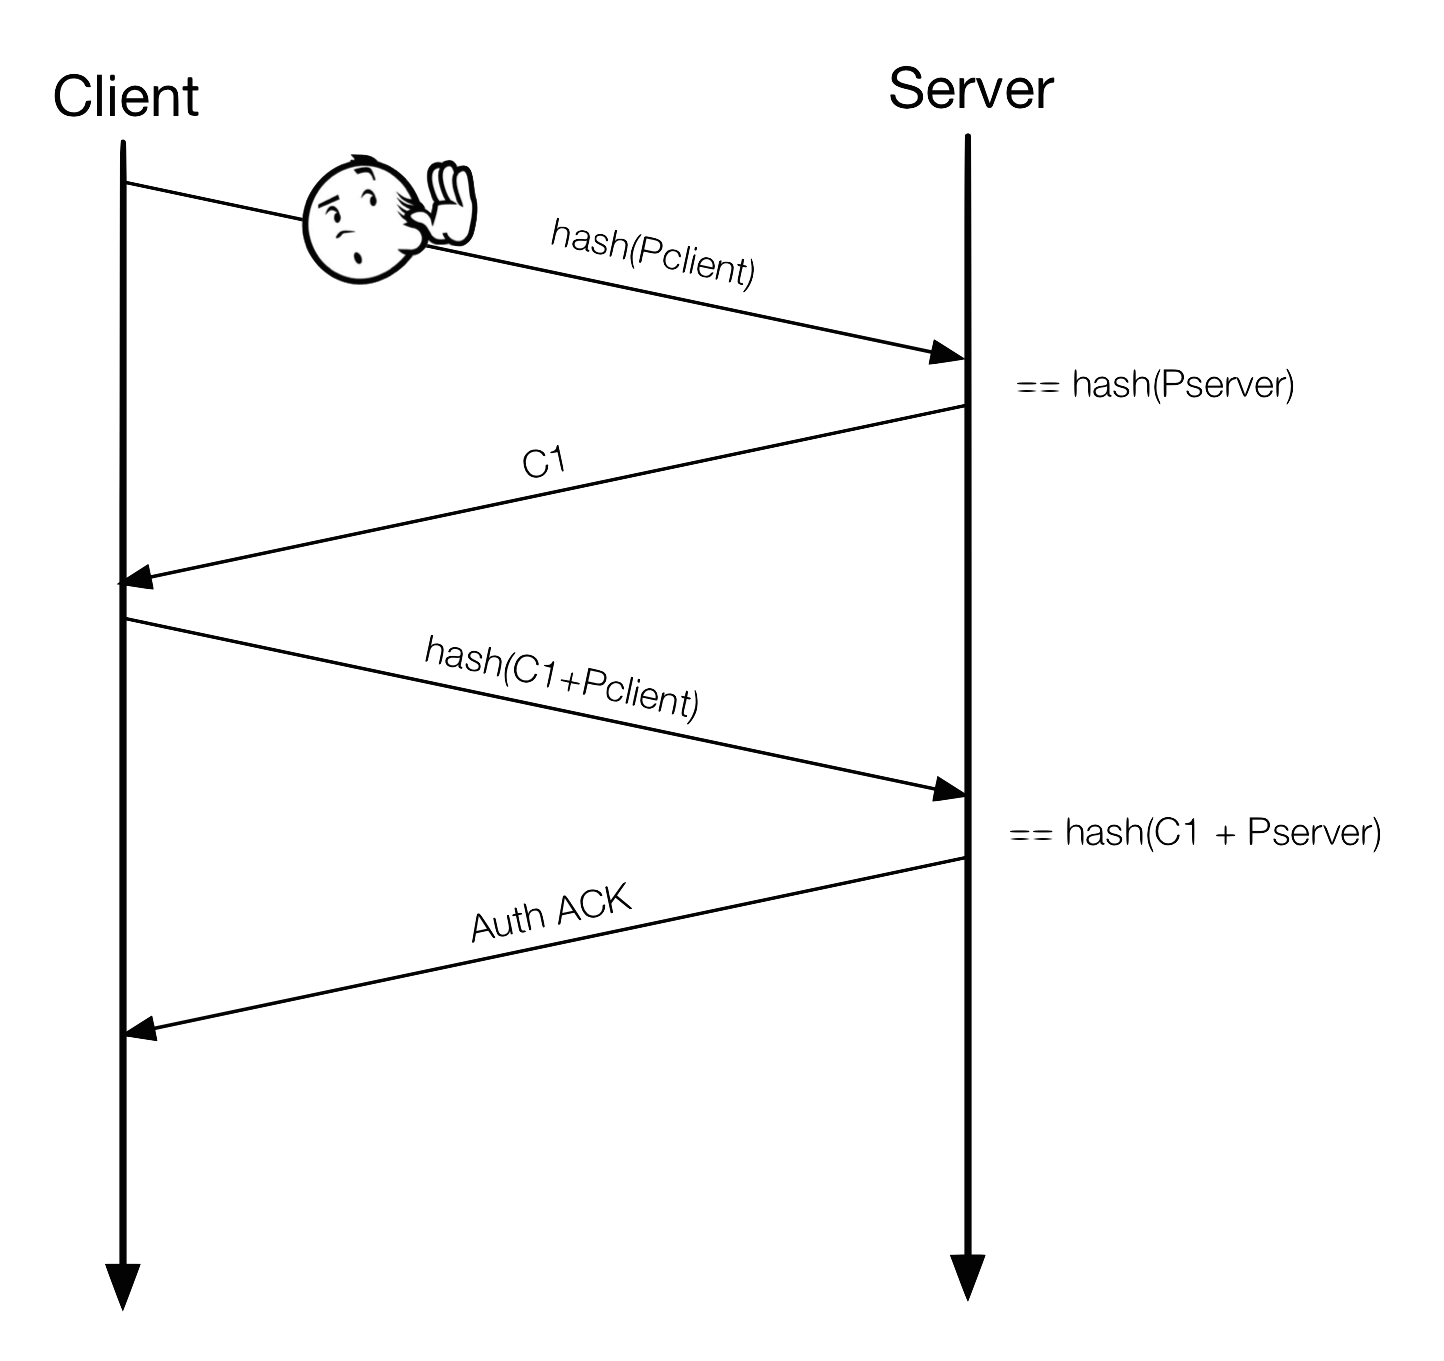
\includegraphics[width=\linewidth]{Images/SniffPassword.png}
	\captionof{figure}{Eavesdrop first attack}
\end{Figure}

The client sends to the server the hash of the secret. This hash is
successfully intercepted by Eve, who wants to impersonate the client.
The protocol implemented avoid the attack because Eve cannot reply
successfully to the request of a challenge sent by the server: the
correct answer is the hash of a combination of the challenge sent
and the plain text of the password, that never is sent on the network.
The attacker cannot in this way act on behalf of the client.

A second example of a possible eavesdropping attack is reported in
figure 4, where Eve successfully eavesdropped the answer the client
gives to a challenge. Also in this second example, Eve cannot reply
to the next challenge, since the next token is new and random-generated.
Again, the attack is prevented because there is no way to know the
secret of the user.

\begin{Figure}
	\centering
	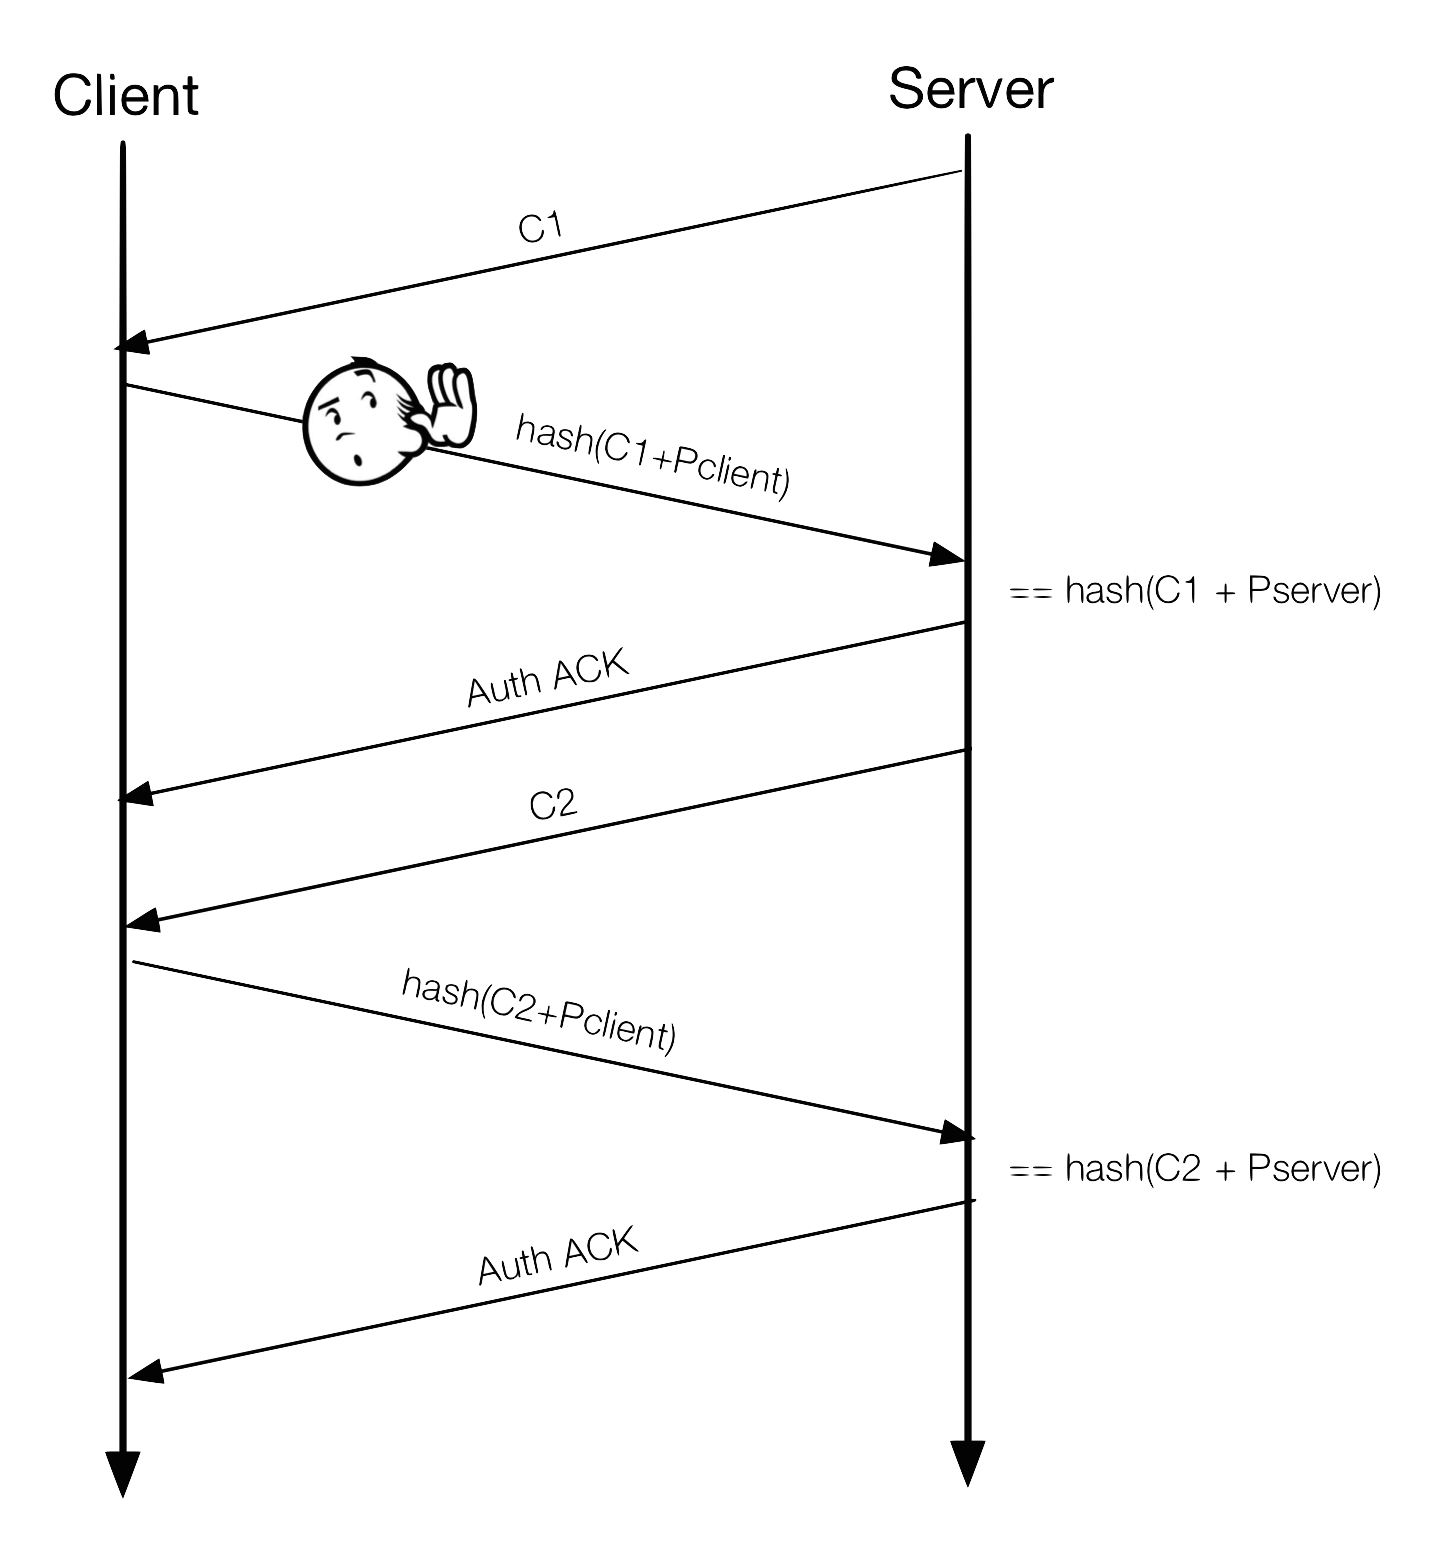
\includegraphics[width=\linewidth]{Images/SniffChallenge.png}
	\captionof{figure}{Eavesdrop second attack}
\end{Figure}

Another importan protection provided by CHAP is that it is possible
to authenticate a client also in non-encrypted channels, since all
the messages are encoded with an hash function. In figure 5 we provide a packet sniffing on the challenge messages performed with Wireshark, and we can see how each important message passing through the network is encoded and not understandable.

\textcolor{red}{FIGURA WIRESHARK??}

\section{Conclusions}

\end{multicols}
\end{document}
